\textbf{La información de los atletas que ganaron medallas en la disciplina halterofilia.}\vspace{.3cm}

Ahora bien, en esta consulta a diferencia de las otras 2, primero accedimos a la información sobre los atletas y las disciplinas en las que ganaron medallas. Por lo tanto, estructuramos nuestra consulta de la siguiente manera: \vspace{.3cm}

\begin{lstlisting}
    SELECT 
    a.IDAtleta,
    a.Nombre,
    a.PrimerApellido,
    a.SegundoApellido,
    a.FechaNacimiento,
    a.Nacionalidad,
    a.Genero,
    m.TipoMedalla
FROM 
    Medalla m
JOIN 
    Atleta a ON m.IDAtleta = a.IDAtleta
JOIN 
    Disciplina d ON m.IDDisciplina = d.IDDisciplina
WHERE 
    d.NombreDisciplina = 'Halterofilia';
\end{lstlisting}

\vspace{.3cm}

Seleccionamos la tabla Medalla y la renombramos como m. Luego, realizamos una unión (JOIN) con la tabla Atleta, renombrada como a, utilizando la columna IDAtleta que es común en ambas tablas. Esta unión nos permite obtener la información de los atletas que han ganado medallas. \vspace{.3cm}

Posteriormente, realizamos otra unión (JOIN) con la tabla Disciplina, renombrada como d, utilizando la columna IDDisciplina que es común en ambas tablas. Esto nos permite acceder a la información sobre las disciplinas en las que se ganaron las medallas.

Aplicamos una cláusula WHERE para filtrar los resultados y seleccionar únicamente las filas donde el nombre de la disciplina sea 'Halterofilia'.

Finalmente, seleccionamos las columnas relevantes de la tabla Atleta (IDAtleta, Nombre, PrimerApellido, SegundoApellido, FechaNacimiento, Nacionalidad, Genero) y la columna TipoMedalla de la tabla Medalla para obtener la información completa de los atletas que ganaron medallas en halterofilia. \vspace{.3cm}

El resultado es una lista detallada de los atletas que han ganado medallas en la disciplina de halterofilia, incluyendo información relevante sobre ellos y el tipo de medalla que ganaron. \vspace{.3cm}

\textbf{Resultado:}
\begin{center}
    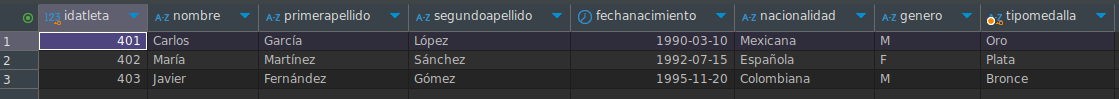
\includegraphics[width=15cm]{resources/resultados/r9.png}
\end{center}   

Tambien, se añadieron manualmente tuplas en la tabla medalla para asegurar que haya registros de medallas en la disciplina de halterofilia. \vspace{.3cm}